\chapter{Opis zastosowanego rozwi\k{A}zania}

Rozdział ten zawiera opis zastosowanego w ramach pracy rozwiązania służącego do zdalnego nadzorowania pracy urządzeń. Rozwiązanie to zostało zaprojektowane dla dwóch typów użytkowników. Pierwszym z nich jest projektant widoków – osoba odpowiedzialna za ich tworzenie, która posiada podstawową wiedzę na temat urządzeń. Drugim typem użytkownika jest osoba upoważniona do oglądania widoków. W żargonie branży kolejowej termin ,,widok'' można zastąpić słowem ,,wizualizacja''.

Rozwiązanie zostało zaimplementowane jako aplikacja internetowa składająca się z dwóch modułów. Każdy z nich przeznaczony jest dla odpowiedniego typu użytkownika. Zadaniem pierwszego modułu aplikacji - ,,Elements Designer'' jest projektowanie widoków. Są to strony złożone z elementów graficznych, które pozwalają na wizualizację stanu urządzenia. Drugi moduł o nazwie ,,Elements Viewer'' służy do wyświetlania tych widoków wraz z nawiązaniem połączenia z urządzeniami i dostarczeniem danych w odpowiednie miejsca wizualizacji. Kolejne podrozdziały zawierają szczegółowy opis funkcjonalności modułów.

\section{Elements Designer - Moduł projektowania widoków}

Moduł Designer pozwala na projektowanie widoków urządzeń. Jego interfejs składa się z dwóch głównych elementów – menu bocznego oraz głównego obszaru roboczego, który prezentuje obecny stan projektu. Obszar ten nosi nazwę ,,sceny''. Dzięki temu rozwiązaniu projektant widzi efekt swojej pracy natychmiast po dokonaniu zmian.
Projektowanie widoku polega na wybieraniu tzw. komponentów z menu bocznego, umieszczaniu ich w odpowiednim miejscu na scenie i konfigurowaniu wedle potrzeb. Interfejs modułu Designer widoczny jest na rysunku \ref{fig:designer_complete}.


\begin{figure}[h]
\centerline{
	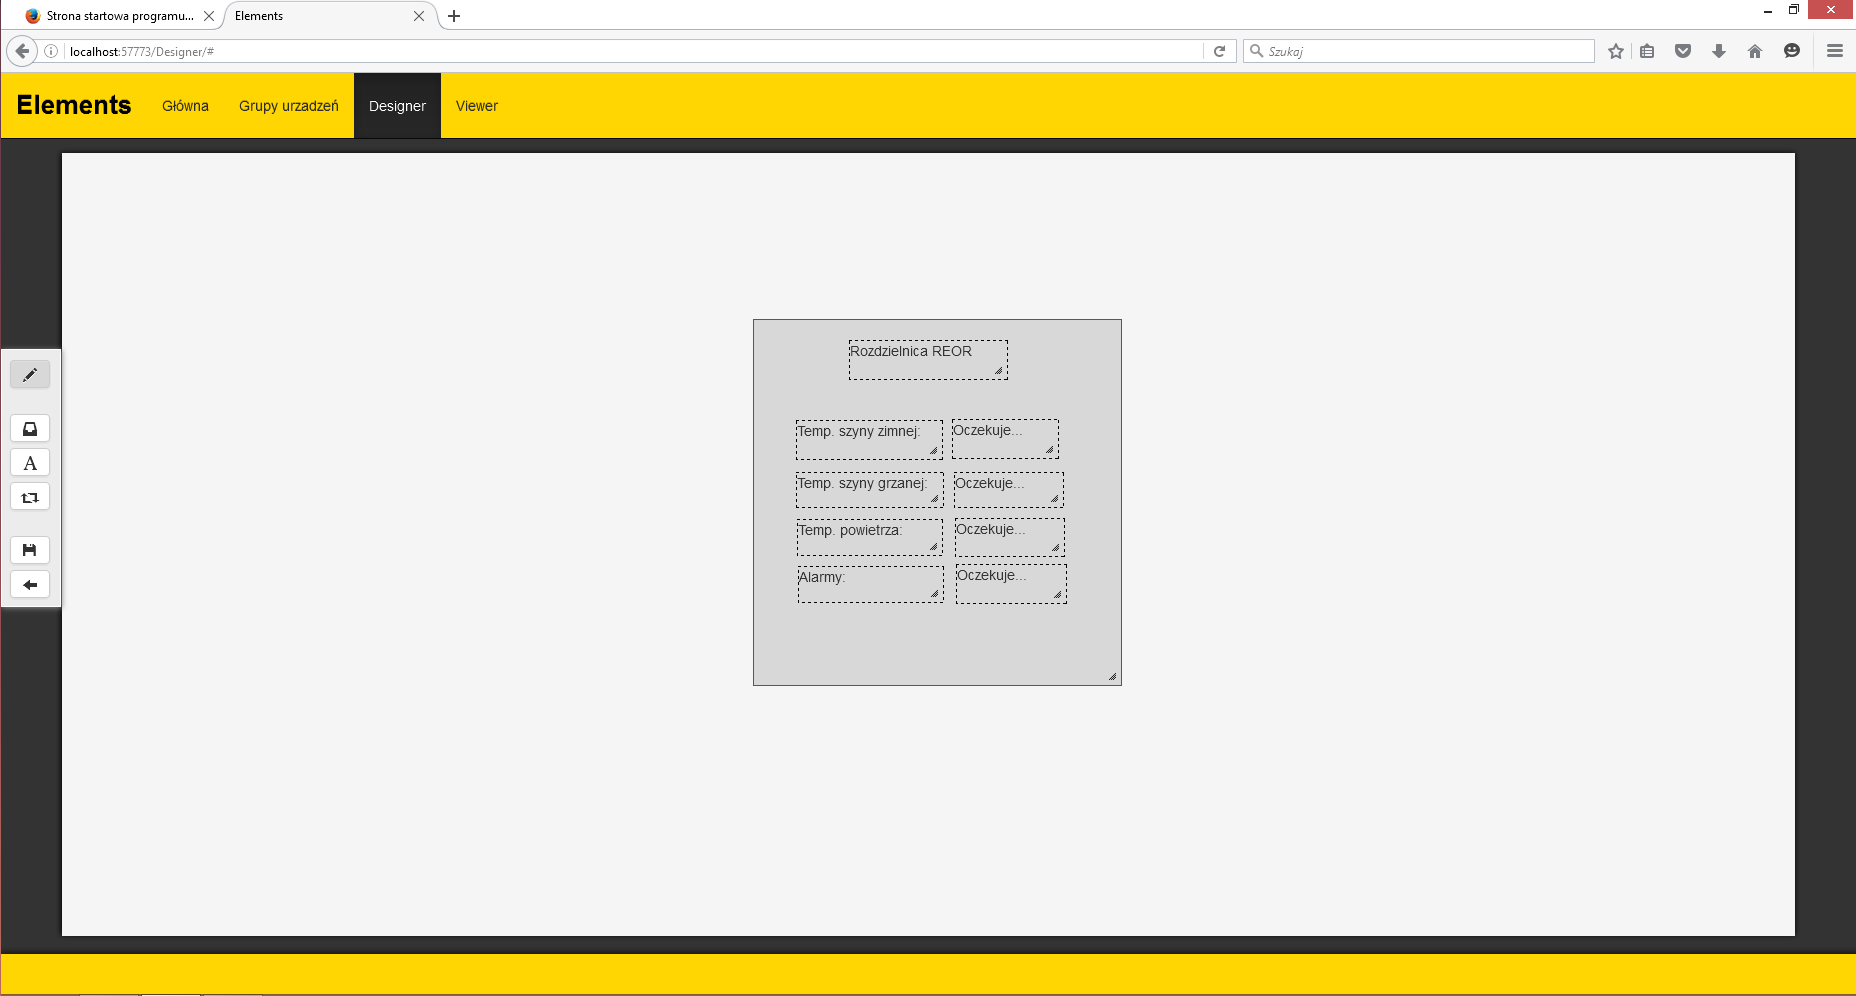
\includegraphics[width=180mm]{./img/screen/designer_projektgotowy.png}
	}
	\caption{Interfejs graficzny modułu Designer}
	\label{fig:designer_complete}
\end{figure}

\subsection{Tworzenie projektu}

Po wybraniu modułu z odpowiedniej sekcji menu aplikacji użytkownikowi ukazuje się strona wyboru projektu. Każdy projekt widoczny jest jako kafelek z nazwą i opisem projektu. Użytkownik może z tego miejsca przejśc do edycji istniejącego projektu lub stworzyć nowy. W takiej sytuacji należy uzupełnić nazwę, opis oraz grupę urządzeń, dla której projektowany będzie widok. Po zatwierdzeniu tych danych użytkownikowi ukazuje się Scena.


\subsection{Scena}
Scena jest obszarem roboczym, który gromadzi wszystkie komponenty. Po zapisaniu projektu, możliwe będzie wyświetlenie jej przez moduł Viewer wraz ze wszystkimi komponentami naniesionymi na nią w trakcie projektowania. Jedynym atrybutem sceny, który można konfigurować jest kolor jej tła.

\subsection{Komponenty}
Komponenty to podstawowe elementy składowe projektu, które pełnią różne funkcje. W praktyce jest to każdy element dodany przez użytkownika do Sceny w trakcie projektowania. Komponenty dodawane są za pomocą przybornika znajdującego się w lewej części interfejsu. Przybornik przedstawiony jest na obrazie \ref{fig:toolbox}. 

\begin{figure}[h]
\centerline{
	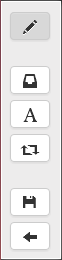
\includegraphics[width=10mm]{./img/screen/designer_przybornik.png}
	}
	\caption{Przybornik}
	\label{fig:toolbox}
\end{figure}


W aplikacji Elements istnieją trzy rodzaje komponentów, które można rozróżnić na podstawie ich funkcji:
\begin{itemize}
	\item Kontener – służy do grupowania innych komponentów. Można w nim umieścić dowolny komponent, ale sam również może być umieszczony w innym kontenerze. Aby umieścić element w kontenerze należy chwycić go myszą i ,,upuścić'' nad wybranym komponentem typu kontener. Czynność tę można odwrócić wybierając opcję ,,Przenieś wyżej'' z menu kontekstowego komponentu.
	\item TextBox – jego funkcja to przechowywanie tekstu, który można edytować. Dzięki temu możliwe jest tworzenie opisów innych elementów projektu. Tekst wpisywany jest podczas tworzenia komponentu. TextBox można edytować w każdej chwili wybierając odpowiednią opcję z jego menu kontekstowego.
	\item RefreshedVariable – element ten powiązany jest z konkretną zmienną urządzenia, którą należy wybrać podczas tworzenia komponentu. Jego główną funkcją jest regularne odświeżanie wartości zmiennej urządzenia w przypadku jej zmiany. Dodatkowo można skonfigurować zmianę tekstu i koloru tła komponentu w chwili gdy wartość zmiennej wyniesie lub przekroczy zdefiniowaną wartość. Pozwala to na zwrócenie uwagi użytkownika na zmienne w wyjątkowych sytuacjach. Można też ustawić komponentowi wartość domyślną. Dzięki temu komponent nie musi wcale zawierać liczby, a jedynie tekst informujący o stanie w jakim znajduje się urządzenie. Okno służące do dodawania komponentowi zdarzeń znajduje się na obrazie \ref{designer-behaviour}. 
	\begin{figure}[h]
	\centerline{
		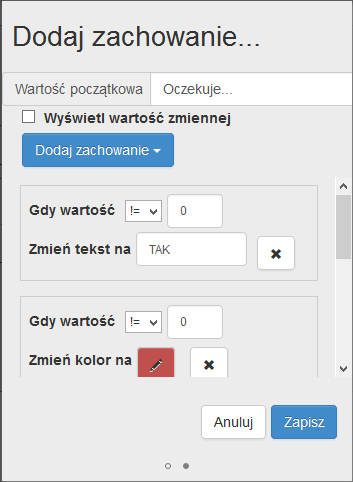
\includegraphics[width=70mm]{./img/screen/designer_zmiennazachowanie.png}
		}
		\caption{Okno dodawania zachowań do komponentów}
		\label{fig:behaviour}
	\end{figure}
	Kolejną opcją jest nałożenie maski bitowej na zmienną. Przed wyświetleniem jej wartości element przemnoży ją przez liczbę ustawioną wcześniej jako maska. Jest to przydatne w przypadku gdy jedną zmienną należy interpretować jako więcej niż jedną liczbę. Ostatnią możliwością jest ustawienie wartości mnożnika. Komponent po prostu przemnoży wartość zmiennej przez mnożnik przed jej wyświetlaniem. W przypadku wybrania przez użytkownika opcji maski bitowej i mnożnika jednocześnie, mnożenie wykonywane jest jako ostatnia operacja.
\end{itemize}

Wszystkie komponenty posiadają dodatkowo kilka wspólnych właściwości, które można konfigurować wedle upodobań. Są nimi kolor tła, kolor obramowania, współrzędne oraz rozmiar. Wszystkie wyżej wspomniane właściwości można zmienić w dowolnej chwili posługując się menu kontekstowym dostępnym pod prawym przyciskiem myszy.  Dla wygody użytkownika rozmieszczenie komponentu określa się przeciągając go po scenie z miejsca na miejsce. Rozmiar natomiast reguluje się chwytając za wybrany narożnik komponentu i rozciągając go.

W momencie gdy użytkownik uzna iż projekt jest już gotowy musi go zapisać, aby zmiany nie zostały utracone. Służy do tego guzik z ikoną dyskietki znajdujący się w menu bocznym. Do edycji można wrócić w każdej chwili wybierając projekt ponownie z listy projektów.


\section{Elements Viewer – moduł wyświetlania widoków}
Moduł Viewer służy do prezentowania widoków użytkownikom końcowym – głównie kolejarzom. Viewer jest w stanie wczytać projekt widoku i wyświetlić go użytkownikowi utrzymując przy tym połączenie z urządzeniami i wyświetlając ich zmienne w skonfigurowany przez projektanta sposób.

\subsection{Lista urządzeń}
Pierwszą stroną, która ukazuje się użytkownikowi po uruchomieniu modułu jest lista wszystkich urządzeń podłączonych do aplikacji Elements. Konfiguruje się ją edytując odpowiedni plik xml w folderze aplikacji. Każde urządzenie na liście reprezentowane jest przez pojedynczy kafelek, który wyświetla jego nazwę. Po kliknięciu na guzik z ikoną lupy użytkownik zostaje przeniesiony do listy projektów dostępnych dla urządzenia.

\subsection{Lista projektów}
Interfejs listy projektów prezentuje się analogicznie do listy urządzeń. Każdy projekt reprezentowany jest przez kafelek z jego nazwą i opisem. Aplikacja przyporządkowuje widoki do urządzeń na podstawie przynależności urządzenia do grupy. Oznacza to, że wiele urządzeń może zostać przeniesionych do tego samego widoku, który wyświetli w nim zmienne wybranego urządzenia.

\subsection{Wizualizacje pracy urządzeń}
Głównym elementem widocznym na stronie projektu jest Scena. Wygląda ona prawie identycznie jak w module Designer. Różnica polega na tym, że menu projektowania jest ukryte. Użytkownik nie może też przesuwać komponentów ani wywołać menu kontekstowego. Widok jest przeznaczony jedynie do oglądania. Moduł Viewer zobrazowany jest na obrazie \ref{fig:viewer_project}.

\begin{figure}[h]
\centerline{
	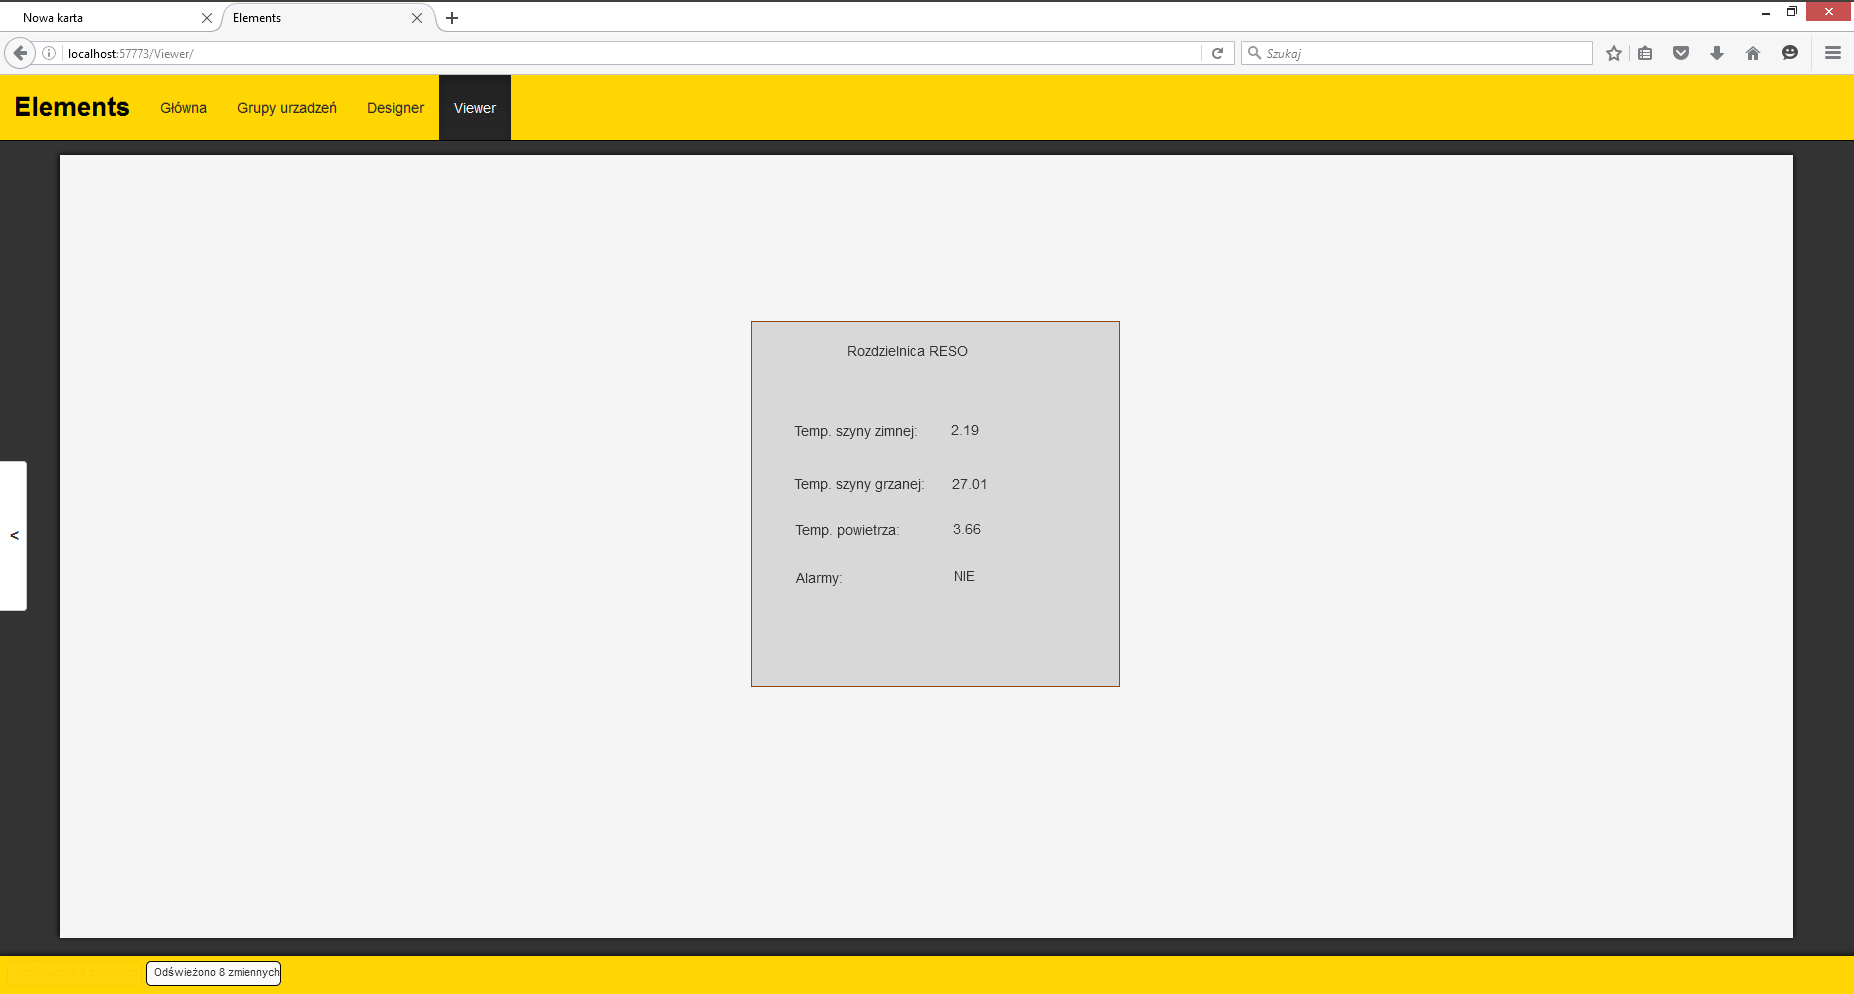
\includegraphics[width=180mm]{./img/screen/viewer_projekt.png}
}
	\caption{Interfejs graficzny modułu Viewer}
	\label{fig:viewer_project}
\end{figure}
	
Po wybraniu projektu użytkownikowi ukazuje się układ komponentów wraz z nadanymi im atrybutami przez projektanta. Aplikacja nawiązuje połączenie z serwerem wymiany danych z urządzeniami w celu uzyskania wartości zmiennych dla komponentów typu RefreshedVariable. Połączenie z serwerem utrzymywane jest przez cały czas, gdy użytkownik znajduje się na stronie projektu. Dzieje się tak, ponieważ aplikacja regularnie kontroluje, czy wartości zmiennych nie uległy zmianie i w takim przypadku aktualizuje je w komponentach. Aktualizacja zmiennej polega na wyświetleniu jej w komponencie RefreshedVariable, który jest z nią związany. Przed wyświetleniem zmiennej aplikacja wykonuje dodatkowe czynności, uwzględniając konfigurację danego komponentu przez projektanta (zmiana tekstu, zmiana koloru, maska bitowa, mnożnik).

